\chapter{Introduction}
\label{cap:introduction}

\section{The Company}
\href{https://www.221e.com/about-us}{221e S.r.l.}\footcite{site:221e}, an innovative startup established in 2012 in Italy, has business units in Padova, Treviso, and Bergamo. The company leverages advancements in IT, microelectronics, sensors, and control algorithms to develop miniaturized wireless embedded systems.

Operating under a dual-layer business model, 221e offers:
\begin{enumerate}
    \item OEM (Original Equipment Manufacturer) services to third-party clients needing a technology partner for product development. This involves R\&D contracts followed by commercial agreements for the supply of engineered systems or technology licensing.
    \item Finished products, particularly general-purpose multi-sensor hardware platforms, to direct customers or distributors.
\end{enumerate}

Targeting the Wearable Devices market and the broader Internet of Things (IoT) industry, 221e capitalizes on the limitless applications within these fields. The name 221e, which represents the infinity Unicode character (\(\infty\)), reflects this boundless potential.

Despite being a small business, 221e is rapidly growing, driven by innovation and entrepreneurship, riding the wave of IoT and wearable device advancements.

\begin{figure}[htbp]
    \centering
    
\includegraphics[height=2cm]{221e_logo.png}
    \caption{221e's logo}
\end{figure}

\begin{figure}[htbp]
    \centering
    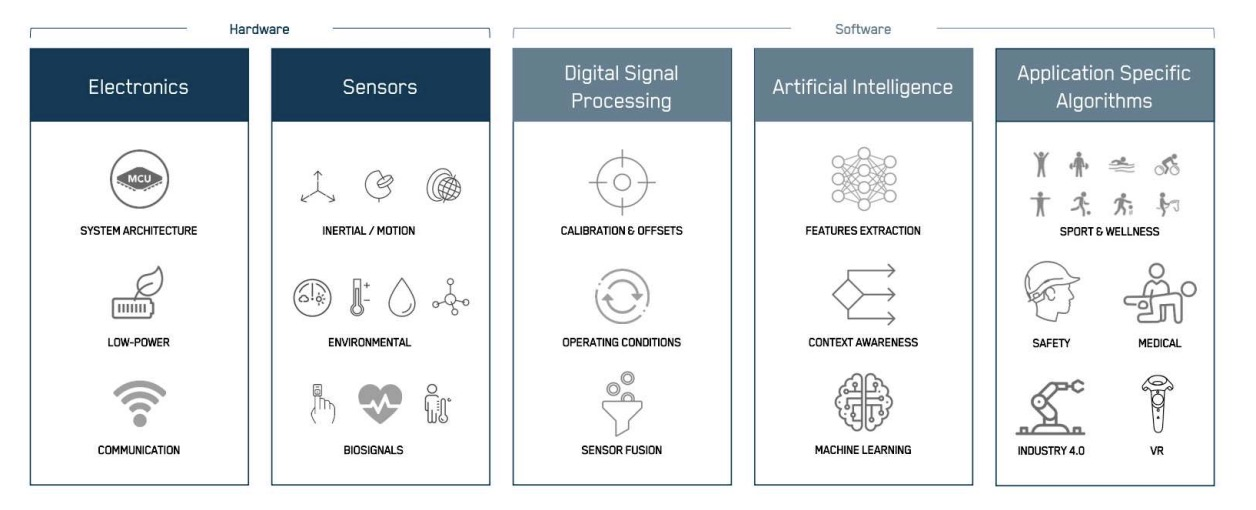
\includegraphics[width=\textwidth]{221e_applications.png}
    \caption{221e's technology echosystem}
\end{figure}


\newpage
\section{Idea}

The idea behind the project is to create a cloud-agnostic architecture for the 221e's IoT devices. The architecture should be able to ingest data from multiple sources, store it and  analyze it. The architecture should be able to scale horizontally and vertically, and should be able to be deployed on multiple cloud providers.


%<\section{Thesis outline}

%\begin{description}
 %   \item[{\hyperref[cap:requirements]{The second chapter}}] describes the high level requirements.
  %  \item [{\hyperref[cap:technologies]{The third chapter}}] describes the technologies taken into consideration for the project.
   % \item[{\hyperref[cap:method]{The fourth chapter}}] describes how the solution has been implemented.
    %\item[{\hyperref[cap:results]{The fifth chapter}}] assess the results of the project.
    %\item[{\hyperref[cap:conclusion]{The last chapter}}] describes the conclusion of the project and the future work.
%\end{description}
